\documentclass[11pt,letterpaper]{article}
\usepackage[margin=0.82in]{geometry}
\usepackage[T1]{fontenc}
\usepackage{lmodern}
\usepackage{microtype}
\usepackage{xcolor}
\usepackage{booktabs,tabularx,array}
\usepackage{tikz}
\usepackage{graphicx}
\usepackage{caption}
\usetikzlibrary{arrows.meta,positioning}
\usepackage[hidelinks]{hyperref}
\usepackage{enumitem}
\setlist[itemize]{leftmargin=1.3em,itemsep=2pt,topsep=3pt}
\definecolor{navy}{HTML}{16324F}
\definecolor{teal}{HTML}{147D83}
\definecolor{pale}{HTML}{EEF5F7}
\usepackage{titlesec}
\titleformat{\section}{\large\bfseries\color{navy}}{\thesection.}{0.55em}{}
\titlespacing*{\section}{0pt}{12pt}{5pt}
\setlength{\parindent}{0pt}
\setlength{\parskip}{5pt}
\newcommand{\service}[1]{\textbf{#1}}
\begin{document}
\begin{center}
{\LARGE\bfseries\color{navy} AWMS Athlete Workload Management Service}\\[4pt]
{\large Cloud-Based Athletic Workload Monitoring and Injury Risk Awareness Service}\\[8pt]
\textbf{Project participants:} Arnav Karnik\\
\textit{Project proposal}
\end{center}

\section{Project Goals}
Develop a cloud-based service that imports activities from Strava and user-uploaded Garmin FIT files, accepts manually entered workouts, and visualizes changes in athletic training volume and intensity. The system will help athletes analyze their workload and recommend resting periods to prevent injury. 

The minimum viable product (MVP) will support athlete authentication, three activity entry methods, independent dated journal entries, exploratory workload analytics, an interactive dashboard, Redis-backed caching of recent metrics, and opt-in SMS alerts when configurable workload thresholds are exceeded.

\section{Specific Software and Hardware Components}
\renewcommand{\arraystretch}{1.18}
\begin{tabularx}{\linewidth}{@{}>{\bfseries}p{0.29\linewidth}X@{}}
\toprule
Component & Technology and role\\ \midrule
Wearable hardware & Garmin watch or cycling computer; optional external heart-rate sensor\\
Activity sources & Strava REST API with OAuth 2.0; Garmin \texttt{.fit} files exported by users; manual workout forms\\
Frontend & React, JavaScript, Recharts; workout entry, journal, preferences, and dashboard screens\\
API/backend & Python 3, FastAPI, Uvicorn, containerized on Google Cloud Run\\
Data processing & Garmin FIT Python SDK, pandas, NumPy; custom workload calculation code\\
Cloud infrastructure & Google Cloud Run, Cloud Storage, Firestore, Pub/Sub, and Memorystore for Redis; optional Cloud Scheduler\\
SMS provider & Twilio Messaging API for opt-in workload alerts\\
Testing and operations & pytest, curl/Postman, GitHub, Google Cloud Logging\\
\bottomrule
\end{tabularx}

\clearpage
\section{Architectural Diagram}
\begin{center}
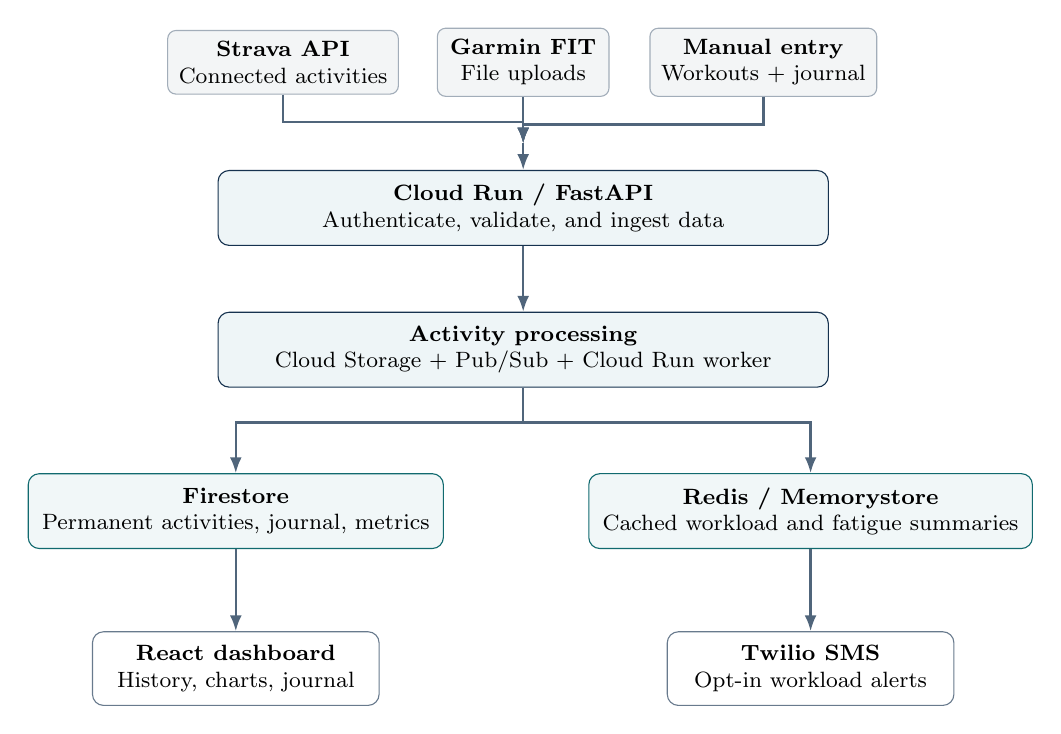
\begin{tikzpicture}[
  font=\footnotesize, >=Latex,
  source/.style={draw=navy!40,fill=navy!5,rounded corners=3pt,minimum width=2.18cm,minimum height=.72cm,align=center,inner sep=4pt},
  core/.style={draw=navy,fill=pale,rounded corners=4pt,minimum width=7.75cm,minimum height=.87cm,align=center,inner sep=5pt},
  data/.style={draw=teal!85!black,fill=teal!6,rounded corners=4pt,minimum width=3.64cm,minimum height=.95cm,align=center,inner sep=5pt},
  output/.style={draw=navy!65,fill=white,rounded corners=4pt,minimum width=3.64cm,minimum height=.9cm,align=center,inner sep=5pt},
  flow/.style={-{Latex[length=2mm]},line width=.85pt,draw=navy!75}
]
% Top row: equal-size input cards.
\node[source] (strava) at (-3.05,0) {\textbf{Strava API}\\Connected activities};
\node[source] (garmin) at (0,0) {\textbf{Garmin FIT}\\File uploads};
\node[source] (manual) at (3.05,0) {\textbf{Manual entry}\\Workouts + journal};
\node[core] (api) at (0,-1.85) {\textbf{Cloud Run / FastAPI}\\Authenticate, validate, and ingest data};
\node[core] (processing) at (0,-3.65) {\textbf{Activity processing}\\Cloud Storage + Pub/Sub + Cloud Run worker};
\node[data] (firestore) at (-3.65,-5.70) {\textbf{Firestore}\\Permanent activities, journal, metrics};
\node[data] (redis) at (3.65,-5.70) {\textbf{Redis / Memorystore}\\Cached workload and fatigue summaries};
\node[output] (dashboard) at (-3.65,-7.70) {\textbf{React dashboard}\\History, charts, journal};
\node[output] (sms) at (3.65,-7.70) {\textbf{Twilio SMS}\\Opt-in workload alerts};
% Merge the three input streams cleanly above the API.
\coordinate (merge) at (0,-1.03);
\draw[flow] (strava.south) -- ++(0,-.35) -| (merge);
\draw[flow] (garmin.south) -- (merge);
\draw[flow] (manual.south) -- ++(0,-.35) -| (merge);
\draw[flow] (merge) -- (api.north);
\draw[flow] (api.south) -- (processing.north);
% Wider gutter between Firestore and Redis; preserve alignment with outputs.
% Split toward durable storage and derived cache.
\draw[flow] (processing.south) -- ++(0,-.44) -| (firestore.north);
\draw[flow] (processing.south) -- ++(0,-.44) -| (redis.north);
\draw[flow] (firestore.south) -- (dashboard.north);
\draw[flow] (redis.south) -- (sms.north);
\end{tikzpicture}
\end{center}

\section{Interaction Between Components}
Athletes authorize Strava, upload exported Garmin FIT files, or manually enter workouts (sport, date, duration, and optional distance, exertion, or notes). FastAPI authenticates requests, stores raw FIT uploads in Cloud Storage, and writes normalized activity metadata to Firestore. Pub/Sub triggers a Cloud Run worker that processes activities and saves workload summaries. Frequently requested derived values, such as the most recent fatigue indicator, seven-day workload, and dashboard summary, are cached in Google Cloud Memorystore for Redis. But most of the atheltic data will be stored in Firestore . On a cache miss, the API reads the stored summary from Firestore and repopulates Redis with a short time-to-live (TTL); new workouts or relevant journal edits invalidate affected keys. Source identifiers and time-based matching reduce duplicate imports from Garmin and Strava.

The journal is \emph{independent of workouts}: users can create entries on any date, including rest days, and reflect on training over several preceding days. Optional fatigue, soreness, recovery ratings, and free-text reflections are stored in Firestore and can be browsed chronologically. Entries may optionally reference past workouts but do not require one.

An alert evaluator checks newly calculated workload metrics against configurable thresholds. If an athlete has opted in, a threshold is exceeded, and a cooldown rule permits delivery, the backend sends an advisory SMS through Twilio. Phone numbers, consent status, and notification history are stored securely. Alerts are informational and suggest considering rest or reduced intensity, not a medical diagnosis. The design will also account for unsubscribe requests and failed deliveries.

\section{Exploratory Athletic Workload Methodology}
The final workload algorithm has \emph{not yet been selected}. We plan to investigate workout duration, frequency, heart rate and heart-rate-zone time, perceived exertion (RPE), distance, elevation gain, and historical training trends. Candidate methods include session RPE (duration multiplied by post-workout exertion), weighted heart-rate-zone load, seven-day and 28-day workload averages, and changes from an individual's baseline. 

\section{Redis Caching Strategy}
The API will use a cache-aside pattern for per-athlete summary values (for example, \texttt{athlete:<id>:fatigue} and \texttt{athlete:<id>:workload7d}). Redis stores only derived, frequently requested results, not the authoritative workout or journal records.

\section{Debugging, Training, and Testing}
\begin{itemize}
\item \textbf{Unit tests:} Verify FIT decoding, manual entry validation, time zones, missing values, duplicate detection, candidate workload formulas, Redis cache hits/misses and invalidation, and alert thresholds/cooldowns.
\item \textbf{Integration tests:} Import FIT files, mock Strava responses and Twilio calls, save independent journal entries, and verify Firestore records, Pub/Sub events, and Redis fallback behavior.
\item \textbf{End-to-end tests:} Import or manually add an activity, create a rest-day journal entry, view updated charts, and trigger a test SMS with explicit opt-in; test errors and retries.
\item \textbf{Cloud debugging:} Use Cloud Logging, structured request/job identifiers, and Pub/Sub delivery diagnostics to trace failed jobs.
\end{itemize}


\section{Four Cloud Technologies and Feasibility}
\begin{itemize}
\item \service{Cloud Run (compute):} Hosts the API and processing worker.
\item \service{Cloud Storage (object storage):} Retains uploaded FIT files.
\item \service{Firestore (managed database):} Stores athlete profiles, activity metadata, and computed metrics.
\item \service{Pub/Sub (messaging):} Decouples activity ingestion from asynchronous processing.
\item \service{Memorystore for Redis (managed caching):} Serves frequently accessed workload and fatigue summaries with low latency, while Firestore retains permanent records.
\end{itemize}

\section{Motivation, Scope, and Limitations}
This project combines my interests in sports technology, wearables, and cloud computing with a practical athlete-facing application. Primary challenges include Strava permissions and rate limits, FIT data variation, incomplete heart-rate records, SMS consent and costs, GPS and health-data privacy, and lack of validated injury labels. Access to user data will be authenticated, API credentials protected, and deletion of imported records supported. 

\vspace{4pt}
{\small\textbf{Documentation:} \url{https://developer.garmin.com/fit/get-the-sdk/} \quad \url{https://developers.strava.com/docs/} }
\end{document}